\documentclass[11pt]{article}

%% Language and font encodings
\usepackage[english]{babel}
\usepackage[utf8x]{inputenc}
\usepackage[T1]{fontenc}

%% Sets page size and margins
\usepackage[a4paper,top=3cm,bottom=2cm,left=3cm,right=3cm,marginparwidth=1.75cm]{geometry}

%% Useful packages
\usepackage{amsmath}
\usepackage{graphicx}
\usepackage{color}
\usepackage[colorinlistoftodos]{todonotes}
\usepackage[colorlinks=true, allcolors=blue]{hyperref}

\usepackage{multirow}
\usepackage{tabularx}

% More packages
\usepackage{authblk}
\usepackage{cite}

\title{Does influenza drive absolute humidity?}
\author{Edward B. Baskerville and Sarah Cobey}
\affil{Department of Ecology and Evolution, University of Chicago}

\begin{document}
\maketitle

Multiple lines of evidence suggest that absolute humidity and school terms affect the timing of influenza epidemics, although the contributions of these and other factors are still unresolved \cite{Bjornstad2016,Shaman2010a,Shaman2010b,Chao2010,Tamerius2015}.
In PNAS, Deyle et al. (2016) applied convergent cross-mapping (CCM) to measure the impact of environmental variables on influenza activity \cite{Deyle2016}. 
The authors concluded that absolute humidity and temperature are not merely correlated with influenza activity but in fact directly or indirectly cause epidemics.

The mathematical basis of CCM involves strict assumptions that may be violated in nature \cite{Sugihara2012}.
Process noise, secular changes in parameters, and other transient dynamics can lead to situations where the underlying attractor is undersampled, causing errors in reconstruction and inference \cite{Cobey2016}.
There are not yet any clear statistical tests to determine when CCM has gone awry.
 
One simple test of the method is whether it correctly predicts that influenza does not drive absolute humidity, temperature, relative humidity, and precipitation.
We used the authors' code to test these interactions for each of the 26 countries shown in Figure 3 of Deyle et al. (2016), with modifications, described below, to support different test assumptions.
Deyle et al. (2016) used surrogate time series with randomized anomalies for each of the environmental variables to construct a null distribution for significance testing.
Initially, we analogously used surrogate time series only for influenza to assess if influenza affected each of these variables.
In 53 of 104 tests, influenza was inferred to drive the environmental variable.
When using surrogate time series for both influenza and the environmental variable, influenza was inferred to drive the environmental variable in 56 of 104 tests (Figure~\ref{fig:bycountry}).
This general result was robust to different transformations of the time series, including
\begin{enumerate}
\item using surrogates for both influenza and the environmental variable, influenza alone, or the environmental variable alone;
\item using simple weekly means instead of fitted splines for the seasonal surrogates;
\item removing all zeros from the influenza time series and restricting analyses to periods when influenza was present;
\item log-transforming influenza incidence; and
\item additionally requiring that the maximum cross-correlation appear at a lag corresponding to the correct directionality in time \cite{Ye2015}.
\end{enumerate}
Summaries of results from different test variants are in Table~\ref{tab:summary}.
More thorough testing with simulated data shows that using CCM with surrogate time series frequently leads to false positives.
Other criteria for causality perform better in some instances, but none is universally reliable in a seasonally forced infectious disease system \cite{Cobey2016}.

Although it may be possible to choose surrogates and transformations to obtain more favorable results, it is clear that more work is needed on the statistical basis of CCM before it can be applied out of the box.
We agree with Deyle et al. (2016) that weather affects the timing of influenza activity, but we do not think that analysis based on CCM supports the correct inference regarding causal direction.

The code for our analysis, along with source data and full results, is at \\ \url{http://github.com/cobeylab/ccm-letter}.

\begin{figure}
\centering
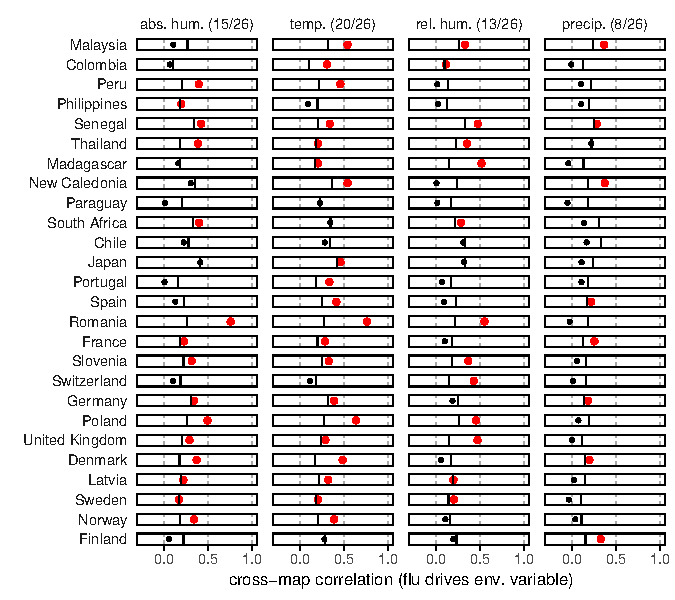
\includegraphics[width=4.5in]{us=1-rz=1-usf=1-use=1-ulf=0-fic=1-lt=0.pdf}
\caption{
    \label{fig:bycountry}
    CCM results testing whether influenza drives environmental variables in different countries.
    Circles show the cross-map correlation; significant interactions are large and red.
    Vertical bars show the location of the 95\% quantile of the null distribution constructed from surrogate time series.
    Surrogates were constructed using splines for both influenza and environmental variables, and analysis was restricted to periods when influenza was present.
    Influenza incidence was not log-transformed.
}
\end{figure}

\begin{table}
\centering
\caption{
    \label{tab:summary}
    Summary of CCM results for whether influenza drives environmental variables, and vice versa, in different countries.
    Tests used surrogates for influenza and/or environmental variables,
    and either untransformed or log-transformed influenza incidence.
    Results are shown with and without the requirement that the maximum cross-correlation occur in the correct temporal direction.
    Surrogates were constructed using splines, and analysis was restricted to periods when influenza was present.
    Numbers are out of a total of 104 tests (26 countries, 4 tests each).
}
\begin{tabularx}{\textwidth}{ c | c | c | c | c | c | c}
\multicolumn{3}{c}{} & \multicolumn{2}{c}{\# sig. of 104} & \multicolumn{2}{c}{\# sig. of 104 (lag test)} \\
\hline
Flu surr. & Env. surr. & Log-flu & flu $\rightarrow$ env. & env. $\rightarrow$ flu. & flu $\rightarrow$ env. & env. $\rightarrow$ flu. \\
\hline
& X &  & 14 & 27 & 8 & 14 \\
X &  &  & 53 & 14 & 25 & 6 \\
X & X &  & 56 & 22 & 27 & 10 \\
& X & X & 17 & 31 & 11 & 15 \\
X &  & X & 55 & 29 & 25 & 13 \\
X & X & X & 52 & 34 & 23 & 15 \\
\end{tabularx}
\end{table}

\bibliographystyle{vancouver}
\bibliography{ccm-letter}

\end{document}